\documentclass{article}
\usepackage[utf8]{inputenc}
\usepackage{amsmath}
\usepackage{graphicx}
\usepackage{hyperref}
\usepackage{tikz}
\usepackage{float}
\usepackage{verbatim}
\usetikzlibrary{automata,positioning}


\title{PDF Lexical Analysis}
\author{Boujamaa ATRMOUH}
\date{\today}

\begin{document}

\maketitle

\section{Introduction}

\begin{flushleft}
    \hspace{1cm}The objective of this project is to develop a series of tools that, given a PDF file, can extract information about its structure. To do this, we will develop different parsers with the aim of analyzing the content of a file. Ideally, these tools should be able to serve as a basis for the development of code that can repair, or even edit, a PDF file.
\end{flushleft}

\section{PDF Structure}


\begin{flushleft}
    \hspace{1cm}Addressing all the subtleties of the PDF format would be far too ambitious, and we will therefore make the following assumptions about the argument file:
    \begin{itemize}
        \item The document is not protected by encryption;
        \item The file contains only one reference table;
        \item This reference table is not compressed;
        \item PDF objects are defined directly in the body of the document (and not within a stream);
        \item Streams never contain the sequence of characters "endstream". This string will therefore always represent the end of stream marker;
        \item Parentheses within PDF character strings are always preceded by the character.
    \end{itemize}
In practice, this means that our code will be able to handle almost all PDF files in version 1.4 (or lower), unencrypted and without incremental modification.
\end{flushleft}

\subsection*{I}

\begin{flushleft}
    \hspace{1cm} Files \texttt{parser1.y} and \texttt{lexer1.l}.
The main program takes as its only argument the path to the file to be analyzed. If this file is not valid, an error message will be displayed. If it is valid, the version of the PDF format and the address of the reference table will be displayed on the standard output.

\begin{itemize}
    \item \texttt{VERSION} is a lexeme to represent comments of the form \%PDF-x,y,
    \item \texttt{LINE} is a lexeme to represent any other line of the file,
    \item \texttt{lines} is a non-terminal symbol, representing a sequence of lines from which the last line must be extracted, verify that it contains only a positive integer, and display this integer.
\end{itemize}

\end{flushleft}

\begin{figure}[H]
    \centering
    \scalebox{.8}{
    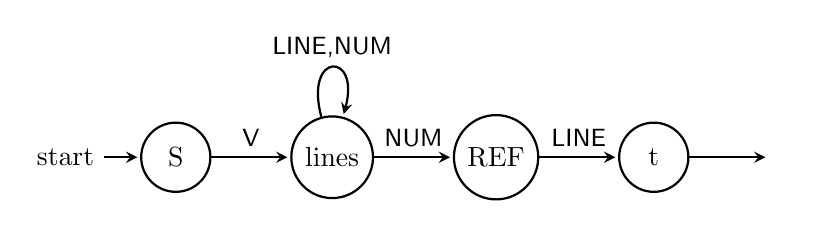
\begin{tikzpicture}[->,>=stealth,shorten >=1pt,auto,node distance=1cm,
        thick,main node/.style={circle,draw,font=\sffamily\Large\bfseries}]
    
    \node[state, initial] (S) {S};
    \node[state] (lines) [right=of S] {lines};
    \node[state] (REF) [right=of lines] {REF};
    \node[state] (t) [right=of REF] {t};
    
    \node[draw=none, right=of t] (dummy) {};
    
    \path[every node/.style={font=\sffamily\small}]
    (S) edge node {V} (lines)
    (lines) edge [loop above] node {LINE,NUM} (lines)
    (lines) edge node {NUM} (REF)
    (REF) edge node {LINE} (t)
    (t) edge [->] (dummy);
    \end{tikzpicture}
    }
    \caption{automata I}
\end{figure}


\begin{figure}[H]
    \centering
    \begin{minipage}[t]{0.45\linewidth}
        \centering
        \[
        S \rightarrow \text{VERSION} \; \text{lines} \; \text{LINE}
        \]
        \[
        \text{lines} \rightarrow \text{NUM} \mid \text{LINE} \; \text{lines} \mid \text{NUM} \; \text{lines}
        \]
        \caption{I: Grammar}
    \end{minipage}
\hfill
    \begin{minipage}[t]{0.45\linewidth}
        \centering
        \[
        S \rightarrow \text{VERSION} \; \text{lines}
        \]
        \[
        \text{lines} \rightarrow \text{LINE} \; \text{lines} \mid \text{NUM} \; \text{lines} \mid \text{LINE} \; \text{endline}
        \]
        \[
        \text{endlines} \rightarrow \text{LINE}
        \]
        \caption{I: Right-linear grammar}
    \end{minipage}
\end{figure}

\[\text{VERSION} = \verb|%PDF-[0-9]+\.[0-9]+|\]
\[\text{LINE} = \verb|[^\n]+|\]
\[\text{NUM} = \verb|[0-9]+|\]

\end{document}